\section{Balancerede Binære Søgetræer}
\hrulefill

\begin{itemize}
\item Operationer på et binært søgetræ
  \begin{itemize}
  \item Trævandring
  \item Søgning på et binært søgetræ
  \item Indsættelse og sletning
  \end{itemize}
\item Rød-sort træ - Balanceret binært søgetræ
  \begin{itemize}
  \item En øvre grænse for højden
  \item Indsættelse
  \item Sletning
  \end{itemize}
\item Krydsende linjesegmenter
\end{itemize}

\newpage
\subsection{Operationer på et binært søgtræ}

\subsubsection{Trævandring}

\begin{theorem}
  Lad $x$ være en rod til deltræ med $n$ knuder, så vil et kald til en trævandringsfunktion e.g. \texttt{INORDER-TREE-WALK($x$)} tage $\Theta(n)$ tid.
\end{theorem}

\begin{proof}
  Det er let at se at det er $\Omega(n)$, da vi skal besøge alle $n$ knuder, så vi mangler bare at vise at den er $Ø(n)$.\\

  Vi siger at prisen for at lave checket ($x \neq$\texttt{NIL}) er $c>0$, så $T(0) = c$. For $n > 0$ lader vi $x$ have to børn, så $x.left.size = k$ og $x.right.size = n - k - 1$, så er tiden for træet
  $$T(n) \leq T(k) + T(n-k-1) + d$$
  Hvor $d > 0$ er tiden det tager for indmaden i algoritmen e.g. \texttt{PRINT}.\\
  
  Vi viser nu $T(n) = Ø(n)$ ved at bruge substitutionsmetoden til at vise $T(n) \leq (c+d)n + c$ ($T(n)$ er det første test plus indmaden for hvert rekursivt kald, plus den sidste test når $n=0$):\\
  Først viser vi base-case
  \begin{align*}
    T(0) &= c \leq (c + d)0 + c\\
         &= c \leq c
  \end{align*}
  Nu antager vi at $T(m) \leq (c+d)m + c$ for $m < n$
  \begin{align*}
    T(n) &\leq T(k) + T(n-k-1) + d \leq (c+d)n + c\\
         &= ((c+d)k + c) + ((c+d)(n-k-1) + c) + d \leq (c+d)n + c\\
         &= ck + dk + c + cn - ck - c + dn - dk - d + c + d \leq (c+d)n + c\\
         &= cn + dn + c  \leq (c + d)n + c\\
  \end{align*}

  Vi har nu vist at $T(n) = \Omega(n)$ og $T(n) = Ø(n)$, ergo $T(n) = \Theta(n)$.
\end{proof}

\subsubsection{Søgning på et binært træ}

\begin{theorem}
  Søgningsoperationerne \texttt{SEARCH, MINIMUM, MAXIMUM, SUCCESSOR,} og \texttt{PREDECESSOR} har alle en køretid på $Ø(h)$ på et binært søgetræ med højde $h$.
\end{theorem}

\begin{proof}
  I \texttt{SEARCH($x$)} kan vi, på grund af binær søgetræsegenskaben, følge en simpel path fra roden til knuden $x$, ved at se om $x$ er større eller mindre end den nuværende knude. Siden en simpel path er $Ø(h)$ er \texttt{SEARCH} $= Ø(h)$.\\

  \texttt{MINIMUM} og \texttt{MAXIMUM} er endnu lettere. På grund af binær søgetræsegenskaben, er den mindste knude bladet længst til venstre, og den største knude er bladet længst til højre. Igen er det en simpel path som er $Ø(h)$.\\

  \texttt{PREDECESSOR} og \texttt{SUCCESSOR} er lidt mere komplicerede. Her udnytter vi også binær søgetræsegenskaben. For at finde den mindste knude der er større end $x$, er der to tilfælde at tage højde for. Hvis $x$ højre deltræ findes, så er den næste knude den mindste knude i højre deltræ, som vi kan finde i $Ø(h)$ tid. Hvis ikke, så går vi iterativt op til vores forælder, indtil vores forælder er et venstre barn af en knude, hvorefter vi returnerer vores bedsteforælder. I værste tilfælde skal vi følge en simpel path fra et blad til roden, hvilket også er $Ø(h)$. Det er symmetrisk at finde den største knude der er mindre end $x$.\\

  Vi har nu vist at alle søgningsoperationer er $Ø(h)$ på et binært søgetræ med højde $h$.
\end{proof}

\subsubsection*{Indsættelse og sletning}

\begin{theorem}
  Vi kan implementerer \texttt{INSERT} og \texttt{DELETE} i $Ø(h)$ tid, på et binært søgetræ med højde $h$.
\end{theorem}

\begin{proof}
  
\end{proof}

\subsection{Rød-sort træ - Balanceret binært søgetræ}
Et rød-sort træ er et binært træ med et ekstra felt i hver knude, dets farve $x.color$ som er enten rødt eller sort, heraf navnet.\\
Et rød-sort træ er et \textbf{balanceret} binært træ, som sørger for at holde en øvre grænse på højden $h$. Det understøtter følgende egenskaber:
\begin{itemize}
\item Hver knude er enten rød eller sort.
\item Roden af træet er sort.
\item Hvert blad er $T.nil$.
\item Hvis en knude er rød, er begge dets børn sorte.
\item For hver knude, alle simple paths ned til et blad indeholder lige mange sorte knuder.
\end{itemize}
Rød-sort træet bruger et \textbf{NIL} felt $T.nil$ til at fungere som alle bladene og som rodens forælder. $T.nil$ har farven sort, så alle blade i træet bliver set som sorte.\\

Vi definerer også en funktion $bh(x)$ på en knude $x$ til at være den knudes \textbf{black-height}, som er antallet af sorte knuder, eksklusiv sig selv, i en simpel path fra $x$ ned til et blad.\\

\subsubsection{En øvre grænse for højden}
\begin{lemma}
  Et rødt-sort træ med $n$ knuder har en højde på højst $2lg(n+1) = Ø(lgn)$
\end{lemma}

\begin{proof}
  Vi starter med at vise, at et deltræ med rod $x$ har $2^{bh(x)}- 1$ knuder. Vi beviser det med induktion på højden af deltræet.\\
  Hvis $h=0$ har vi at $x$ må være et blad og deltræet under $x$ har derfor
  $$2^{bh(x)} - 1 = 2^o - 1 = 1 - 1 = 0$$
  knuder under sig.\\

  Hvis $h > 0$, er $x$ roden til et deltræ og har to børn, som hver især har enten $bh(x)$ eller $bh(x) - 1$, hvis de er henholdsvis røde eller sorte. Det betyder også, at hvert af børnenes deltræer har mindst $2^{bh(x)-1}-1$ knuder under sig, og $x$ har derfor
  $$(2^{bh(x)-1} - 1) + (2^{bh(x)-1} - 1) + 1 = 2^{bh(x)} - 1$$
  knuder under sig, og vi har nu vist den første påstand.\\

  For at færdiggøre beviset, lad vi højden af træet være $h$. Ifølge den 4. rød-sort egenskab, er mindst halvdelen af knuderne, eksklusiv roden, i en simpel path ned af træet, sorte. Derved er $bh(x)$ af roden $x$ mindst $\frac{h}{2}$, og vi har derfor
  \begin{align*}
           n &\geq 2^{\frac{h}{2}} - 1\\
       n + 1 &\geq 2^{\frac{h}{2}}\\
     lg(n+1) &\geq \frac{h}{2}\\
    2lg(n+1) &\geq h
  \end{align*}

  Ergo har vi vist at højden er $h$ er højst $2lg(n+1)$ og derved $h=Ø(lgn)$.
\end{proof}

Ved at vise at rød-sort træer har en øvre grænse på højden af $Ø(lgn)$, betyder det, at alle operationer på et binært træ der havde $Ø(h)$ har nu en køretid på $Ø(lgn)$.

\subsubsection{Rotation}
Rotation er en ombytning af pointere, som bruges til at opretholde rød-sort egenskaber efter en indsættelse eller sletning.


\begin{center}
    \begin{tikzpicture}[>=latex, every node/.style = {shape=circle, draw, align=center}, level distance=1cm]
      \node(A) at (0, 0) {$y$}
      child{ node {$x$}
        child { node[draw=none] {$\alpha$} }
        child { node[draw=none] {$\beta$} }}
      child{ node[draw=none] {$\gamma$} };

      \node(B) [right=5cm of A] {$x$}
      child { node[draw=none] {$\alpha$} }
      child { node {$y$}
        child { node[draw=none] {$\beta$} }
        child { node[draw=none] {$\gamma$} }};

      \draw[dashed, ->] (A) -- node[draw=none, label=above:Left-rotate] {} (B);
    \end{tikzpicture}
\end{center}

Intuitionen for hvorfor man må rykke på pegerne kan ses her.\\
Nedenfor ses et diagram af forholdene mellem knuderne $x, y$ og deltræerne $\alpha, \beta, \gamma$. Pilene er en peger til en knudes børn. Så længe en peger for en knudes højre barn, peger til en knude til højre, og vice versa for venstre peger, så kan man rykke rundt på pegerne.
\begin{center}
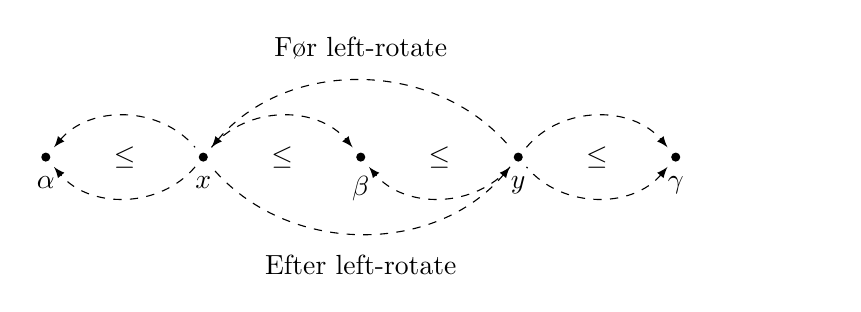
\begin{tikzpicture}[>=latex]
  \draw[draw=none] (0,0) --
  node(A)[pos=.0, label=below:{$\alpha$}] {}
  node [pos=.1] {$\leq$} 
  node(B)[pos=.2, label=below:{$x$}] {}
  node [pos=.3] {$\leq$}
  node [pos=.4, label={[label distance=1cm]above:{Før left-rotate}}] {}
  node [pos=.4, label={[label distance=1cm]below:{Efter left-rotate}}] {}
  node(C)[pos=.4, label=below:{$\beta$}] {}
  node [pos=.5] {$\leq$} 
  node(D)[pos=.6, label=below:{$y$}] {}
  node [pos=.7] {$\leq$} 
  node(E)[pos=.8, label=below:{$\gamma$}] {}
  (10,0)
  ;

  \draw[fill, ]
  (A) circle [radius=0.05]
  (B) circle [radius=0.05]
  (C) circle [radius=0.05]
  (D) circle [radius=0.05]
  (E) circle [radius=0.05]
  ;
  % før
  \draw[dashed, <-] (A) to[bend left=50] (B);
  \draw[dashed, ->] (B) to[bend left=50] (C);
  \draw[dashed, <-] (B) to[bend left=50] (D);
  \draw[dashed, ->] (D) to[bend left=50] (E);
  % efter
  \draw[dashed, ->] (B) to[bend left=50] (A);
  \draw[dashed, <-] (D) to[bend left=50] (B);
  \draw[dashed, ->] (D) to[bend left=50] (C);
  \draw[dashed, <-] (E) to[bend left=50] (D);
\end{tikzpicture}
\end{center}

Right-rotate er den inverse af left-rotate.
\subsubsection{Indsættelse}
Vi kan indsætte i $Ø(lgn)$ tid, med en lille ændring i algoritmen. Ved kald af \texttt{INSERT($T,z$)} indsætter vi $z$ i vores træ som normalt og giver den en rød farve $z.color=red$. Derefter bruger vi en hjælpe funktion \texttt{RB-INSERT-FIXUP}, som sørger for at træet stadig overholder rød-sort egenskaberne efter indsættelse.\\



\subsubsection{Sletning}

\subsection{Krydsende linjesegmenter}
Hvis man har en mængde linjesegmenter og man ønsker at finde ud af om nogen af linjesegmenterne krydser hinanden kan man bruge en metode kaldet \textbf{sweeping}.\\
Sweeping algoritmen bruger en lodret \textbf{sweep line} som kører over mængden af linjesegmenter, og vi betegner den dimension som sweep line bevæger sig over, $x$-aksen, en dimension af tid. Vi antager to ting om vores linjesegmenter, ingen af linjesegmenterne er lodrette linjer, og højst to linjesegmenter kan overlappe på et punkt.\\

Vi bestemmer en relation $\succeq$ mellem to segmenter $s_1$ og $s_2$ i forhold til deres $y$ position ved et bestemt tidspunkt. Vi siger at $s_1 \succeq_x s_2$, hvis $s_1$ ligger højere end $s_2$ ved tidspunkt $x$.
\begin{figure}[H]
  \centering
  \caption{Linjesegmenter og sweep line ved tidspunkt $x_1$ og $x_2$}
  \begin{tikzpicture}
    \draw[dashed] (0.5 , 4) -- (0.5,-1) node[below] {$x_1$};
    \draw[dashed] (3 , 4) -- (3,-1) node[below] {$x_2$};
    \draw (0,1) -- (3.5,1.5) node[anchor=north] {$s_2$};
    \draw (0,2) -- (4, 0) node[anchor=north] {$s_1$};
  \end{tikzpicture}
\end{figure}

Som kan ses på figur 2, så er $s_1 \succeq_{x_1} s_2$ og $s_2 \succeq_{x_2} s_1$.\\
Vi holder styr på forholdene mellem alle segmenterne, i en rangeret orden. Et segment kommer med i ordenen når sweep line passere segmentets venstre ende, og den bliver taget ud af ordenen når sweep line passere dens højre ende.\\

Når to linjesegmenter krydser hinanden kan det ses på deres forhold før og efter sweep line har passeret deres krydsningspunkt. Hvis vi har to segmenter $e, f$, så vil $e \succeq_v f$, hvor $v$ er tidspunket før krydset, og $f \succeq_w e$, hvor $w$ er tidspunktet efter krydset. Præcis i krydsningspunktet vil både $e \succeq f$ og $f \succeq e$.\\

Selve sweep algoritmen sorterer alle linjesegmenterne i forhold deres ender, således at de venstre endepunkter kommer før de højre, hvis de er ens så kommer den med laveste $y$-værdi først. Vi holder styr på dette i et rød-sort træ, hvor, når vi sammenligner knuder i træet, laver vi krydsprodukt mellem to linjesegmenters endepunkter.\\

Algoritmen til at finde krydsende linjesegmenter bruger 4 hjælpefunktioner til rød-sort træet:
\begin{itemize}
\item \texttt{INSERT($T,s$)} indsætter linjesegment $s$ i træet $T$
\item \texttt{DELETE($T,s$)} fjerner linjesegment $s$ fra træet $T$
\item \texttt{ABOVE($T,s$)} returnere linjesegmentet over $s$, således at $s' \succeq s$
\item \texttt{BELOW($T,s$)} returnere linjesegmentet under $s$, således at $s \succeq s'$
\end{itemize}

\begin{algorithm}[H]
  \caption{Algoritme der finder krydsende linjesegmenter}
  \begin{algorithmic}[1]
    \State $S$ en mængde af $n$ linjesegmenter
    \Function{ANY-SEGMENTS-INTERSECT}{$S$}
    \State $T =$ Rød-sort træ
    \State Sorter alle linjesegmenternes endepunkter, venstre før højre, lavest før højest.
    \For{\textbf{each} endepunkt $p$ i den sorterede liste}
    \If{$p$ er venstre endepunkt af linjesegment $s$}
    \State INSERT($T,s$)
    \If{(ABOVE($T,s$) findes og krydser $s$) \textbf{or} (BELOW($T,s$) findes og krydser $s$))}
    \State \textbf{return} TRUE 
    \EndIf
    \EndIf
    \If{$p$ er højre endepunkt af linjesegment $s$}
    \If{både ABOVE($T,s$) og BELOW($T,s$) findes, og ABOVE($T,s$) krydser BELOW($T,s$)}
    \State \textbf{return} TRUE
    \EndIf
    \State DELETE($T,s$)
    \EndIf
    \EndFor
    \State \textbf{return} FALSE
    \EndFunction
  \end{algorithmic}
\end{algorithm}
%%% Local Variables:
%%% mode: latex
%%% TeX-master: "master"
%%% End:
